
The simplest non-constant distribution of connection probabilities is distribution that takes two values $x$, $y$ with probability $p$ and $1-p$ respectively. Formally, let $x, y \in [0,1]$ with $x \neq y$  and $0 < p < 1$. Then, a random variable $X$ follows the two-point distribution \cc{(\enquote{Zweitpunktverteilung}, \href{https://de.wikipedia.org/wiki/Zweipunktverteilung}{Wiki})} $T_{p,x,y}$  if $P(X=x)=p$ and $P(X=y) = 1-p$. 

In a network with connection probabilities $P_{ij}$ distributed after $T_{p,x,y}$ the overall connection probability $\mu$ is
\[
\mu = \E(P_{ij}) = px + (1-p)y.
\]
%% Given $\mu$,$x$ and $y$, the probability $p$ calculates as
%% \begin{align}
%%   p = \frac{c-y}{x-y}. \label{eq:bd1}
%% \end{align}
Assume again, that the with $P_{ij} = P_{ji}$ .The expected overrepresentation of bidirectional connections $\sigma$ is given by
\begin{align}
  \sigma = \frac{\E(P_{ij}^2)}{\mu^2} = \frac{p x^2 + (1-p) y^2}{\mu^2} \label{eq:bd2}
\end{align}
Using \eqref{eq:bd1}, equation~\eqref{eq:bd2} can be reduced to three parameters. It's the question which parameters and how to explore the parameter space.

For example, one can write:
\[
\sigma = \frac{x+y}{\mu} - \frac{xy}{\mu^2}.
\]
See: \href{https://www.wolframalpha.com/input/?i=Simplify[%28%28%28c-y%29%2F%28x-y%29%29*x^2%2B%281-%28%28c-y%29%2F%28x-y%29%29%29*y^2%29%2Fc^2]}{Wolfram Alpha}.

\begin{figure}[h!]
\centering
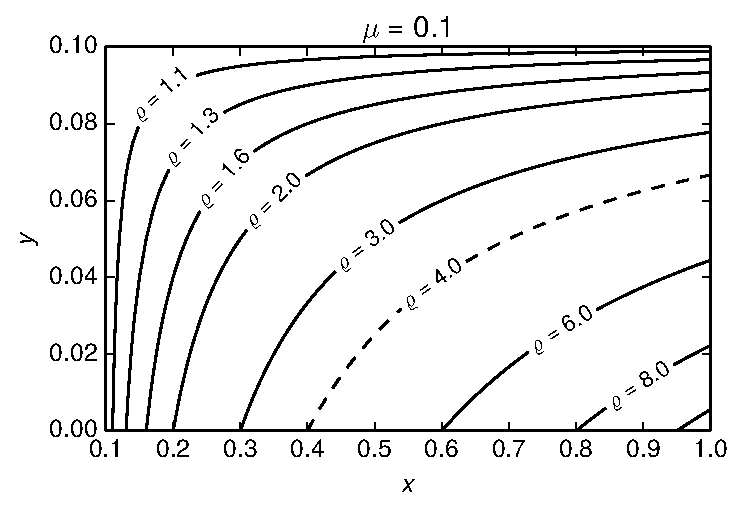
\includegraphics[width=0.6\textwidth]{../lab/two_point_distribution/contour_plot.png}
\caption{Contour plot shows different pairings}
\end{figure}



